%! TEX root = ../listas_completas.tex
\section{Lista 5}
\subsection{E 3.2}
Um aprimoramento do projeto original da plataforma de pesagem é
mostrado aqui com dois amortecedores viscosos que foram introduzidos
limitando para 4 a razão entre amplitudes positivas sucessivas da vibração
vertical na condição descarregada. Determine o coeficiente de
amortecimento viscoso c para cada um dos amortecedores. Admita $m=\SI{4000}{\kilogram}$
e $k=\SI{474}{\kilo\newton\per\meter}$.
\begin{figure}[ht]
    \centering
    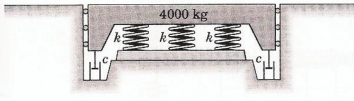
\includegraphics[width=0.4\textwidth]{imagens/questao_3.2.png}
    %\caption{}
    \label{fig:questao3_2}
\end{figure}
\resol
\[k_{eq}=k_1+k_2+k_3 = \SI{1422}{\kilo\newton\per\meter}\]
\[
c_{c}=2\sqrt{k\cdot m} = 2\cdot\sqrt{1422\cdot 10^{2}\cdot 4000}
\]
\[ c_{c} = \SI{1,51d5}{\kilogram\per\second} \]
Como a questão diz que $\zeta = 4$, temos:
\[\zeta=\frac{c_{eq}}{c_{c}} \to c_{eq} = 4 \times 1,51\times 10^{5}
\]
\[
c_{eq}= \SI{6,03d 5}{\kilogram\per\second}
\]
Como há dois amortecedores, para determinarmos o coeficiente de amortecimento viscoso
para cada um, basta dividirmos por dois:
\[
    c = \frac{c_{eq}}{2} = \frac{6,03\times 10^{5}}{2} = \SI{3,02d 5}{kg /s}
\]
\subsection{E 3.4}
 Determine o valor do coeficiente de amortecimento c para o qual o
sistema é criticamente amortecido se $k = \SI{70}{\kilo\newton\per\meter}$ e $m=\SI{100}{kg}$.

\begin{figure}[ht]
    \centering
    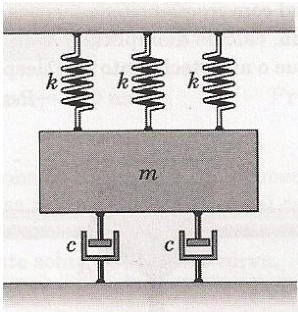
\includegraphics[width=0.25\textwidth]{imagens/questao_3.4.png}
    %\caption{}
    \label{fig:}
\end{figure}

\resol

\[
k_{eq}=70+70+70 = \SI{210}{\kilo\newton\per\meter}
\]
\[
c_{c}=2\cdot\sqrt{210\times 10^3 \times 100} = \SI{9165,1}{\kilogram\per\second}
\]
Como o sistema é \textbf{criticamente} amortecido, temos que $\zeta = 1$
\[ \zeta = \frac{c}{c_c} \]
Logo, o coeficiente de amortecimento ($c$) será igual ao coeficiente de amortecimento
crítico ($c_c$)

Como os amortecedores estão associados em paralelo, temos:
\[
c_{eq} = c_1+c_2
\]
Como $c_1=c_2=c$:
\[
c=\frac{9165,1}{2} = \SI{4582,5}{\kilogram\per\second}
\]

\subsection{E 3.6}
Determine o valor do coeficiente de amortecimento viscoso c para o qual o
sistema mostrado na figura apresenta uma taxa de amortecimento de
\begin{enumalpha}
    \item $0,5$
    \item $1,5$
\end{enumalpha}
\begin{figure}[ht]
    \centering
    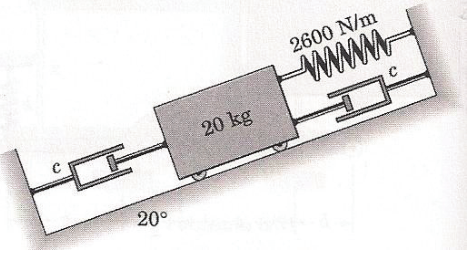
\includegraphics[width=0.3\textwidth]{imagens/questao_3.6.png}
    %\caption{} \label{fig:}
\end{figure}

%\clearpage
\resol

Apesar do conjunto massa + amortecedor estar em um plano inclinado, não haverá
diferença no cálculo do amortecimento, uma vez que a força atuante não é pertinente pois
as equações utilizam apenas a massa.

\begin{minipage}{0.4\linewidth}
\textbf{item a)}
\begin{align*}
    \zeta &= \frac{c}{c_c}\\
    0,5& =\frac{c}{456,07}\\
    c &= \SI{228}{\kilogram\per\second}
\end{align*}
\end{minipage}
\begin{minipage}{0.4\linewidth}
\textbf{item b)}
\begin{align*}
    \zeta &= \frac{c}{c_c}\\
    1,5&=\frac{c}{456,07}\\
    c &= \SI{684}{\kilogram\per\second}
\end{align*}
\end{minipage}
